\subsection{Seleccionar los campos climáticos}
\subsubsection*{Selección y justificación física}
Se obtuvo una base pública de campos globales mensuales: SST NOAA ERSSTv5, presión al nivel del mar (SLP) y altura geopotencial a 500 hPa (Z500) de NCEP/NCAR Reanalysis 1. Se añade presión de superficie como control vertical. La malla nativa de 2$^\circ$/2,5$^\circ$ resuelve patrones de gran escala y evita interpolar a una resolución aparente mayor. No resuelve el relieve ni los procesos de lluvia de una cuenca andina. La selección se fijó antes de calcular mapas de correlación.

\subsubsection*{Mecanismos relevantes y alcance}
Para el occidente y los Andes colombianos, la literatura describe conexiones de la lluvia con SST del Pacífico y Atlántico, ENSO y circulación asociada a los chorros de Chocó y del Caribe (Poveda y Mesa, 1997; Poveda et al., 2014). Es una justificación regional, no una atribución demostrada para La Vieja. SLP y Z500 describen el estado de circulación; para evaluar directamente advección de humedad se necesitarían vientos y humedad, no inferirla solo de estos dos campos.

\subsubsection*{Productos atmosféricos y alternativas}
Se consideraron los productos mensuales ERA5 en superficie y en niveles de presión, distribuidos por el CDS en una malla atmosférica regular de 0,25$^\circ$. En este análisis se adopta NCEP/NCAR Reanalysis 1, de acceso público y resolución de 2,5$^\circ$, como base inicial para identificar patrones de gran escala. ERA5 constituye una alternativa para evaluar la sensibilidad de los resultados al reanálisis y a la resolución espacial; esa comparación requeriría una agregación consistente por área y debe conservar ambos productos separados. La temperatura ERA5-Land utilizada en el estudio de cuenca no reemplaza los campos atmosféricos globales.

\subsubsection*{Periodo, cobertura y correspondencia con la cuenca}
Cada campo descargado contiene 504 meses consecutivos entre enero de 1981 y diciembre de 2022. CHIRPS y Q tienen 485 meses completos; IMERG tiene 300 desde 1998. La comparación principal conserva los mismos 285 meses completos de CHIRPS, IMERG y Q en 1998-2022, con 15 huecos sin relleno. El análisis secundario CHIRPS-Q podrá usar 1981-2022 por separado. La muestra principal aporta entre 22 y 25 pares por mes calendario; los mapas informarán el tamaño efectivo en cada píxel.

\subsubsection*{Unidades, máscaras y transformaciones}
Las medias mensuales no se suman. SLP y presión superficial vienen en las unidades declaradas en el NetCDF: se dividen por 100 solo si están en Pa; millibars equivale a hPa. NCEP hgt ya es altura geopotencial en metros: no se vuelve a dividir por g. En ERA5, geopotential es $\Phi$ en m$^2$/s$^2$ y se convertiría a Z=$\Phi$/9,80665 m. Se conservan los faltantes oceánicos/terrestres de ERSST sin interpolarlos. Las longitudes se normalizan a [-180$^\circ$,180$^\circ$) sin duplicar la costura; cada campo mantiene su malla nativa.

\subsubsection*{Control vertical y máscara para los mapas}
Se comparó cada celda y mes de presión superficial con 500 hPa: se enmascaran 24 valores celda-mes de Z500 donde la presión superficial mensual es menor de 500 hPa. Es un control sobre medias, no garantiza que el nivel esté sobre el terreno durante cada instante del mes. Los mapas por mes calendario deberán conservar solo píxeles con al menos 20 pares y variación no nula. SLP es una reducción al nivel del mar y puede ser menos fiable sobre terreno elevado; se contrastarán sus patrones sobre océanos y tierras altas en 5.3. Los valores de SST próximos a congelación y el hielo marino requieren cautela; el interés físico principal es tropical.

\subsubsection*{Anomalías y muestra de análisis}
Las anomalías de cada campo se definen como la diferencia entre el valor mensual y la media de su mes calendario. La climatología de referencia se estima con las mismas 285 fechas completas de la cuenca durante 1998-2022, de modo que las comparaciones no dependan de calendarios distintos. Los campos conservan su malla nativa, sus unidades y sus faltantes; no se elimina la tendencia. La verificación de una media de anomalías próxima a cero en cada mes confirma esta transformación. Los índices Niño 3.4 u ONI podrán complementar la interpretación, sin sustituir los campos espaciales. La asociación con lluvia y caudal, sus rezagos y su robustez se evaluarán en los apartados siguientes.

\subsubsection*{Procedencia y alcance de los productos}
La base global combina ERSSTv5 y NCEP/NCAR Reanalysis 1, distribuidos por NOAA PSL. ERSSTv5 es una reconstrucción de SST basada en observaciones oceánicas, mientras que los campos atmosféricos proceden de un reanálisis; por ello, sus valores no se interpretan como mediciones locales directas. Se fijaron las versiones, el periodo y los niveles verticales antes de construir los mapas. Los metadatos de soporte conservan las solicitudes de acceso, fechas, coordenadas, unidades y huellas SHA-256 de los archivos, junto con los conteos y las máscaras. La lluvia de Zaragoza no se utiliza como respuesta principal: sus 14 meses completos resultan insuficientes para estimar asociaciones por mes calendario.

\begin{figure}[H]\centering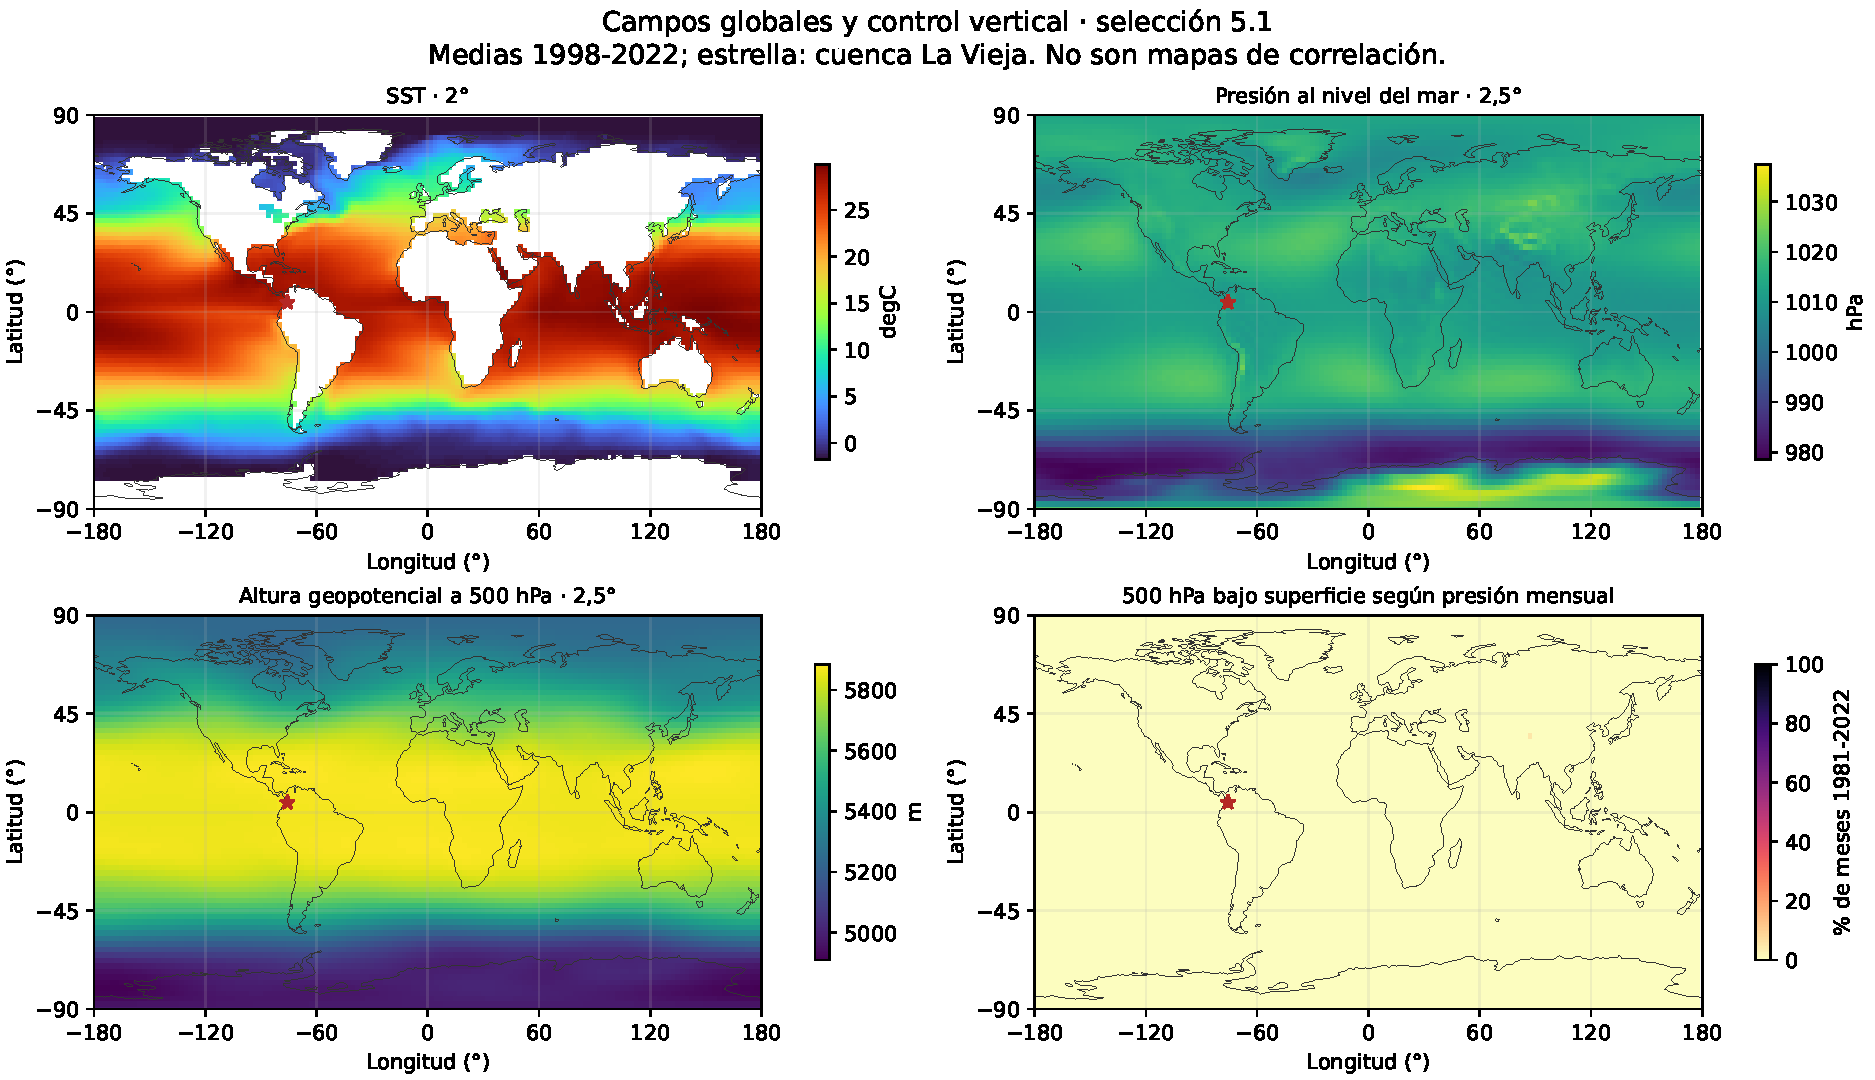
\includegraphics[width=\linewidth]{../apartado_5_1/campos_globales_control.pdf}\caption{Campos obtenidos y control vertical; no son mapas de correlación.}\end{figure}
